\chapter{Clean Architecture}
\label{ch:Clean_Architecture}

Die \textbf{Clean Architecture} hilft bei der Entwicklung von Systemen ohne externe Abhängigkeiten, wie zum Beispiel Frameworks oder User-Interface.
Wie bei vielen anderen Entwurfsprinzipien geht es dabei vor allem darum, Systeme zu entwickeln, die einfach wartbar und erweiterbar sind.
Die Clean Architecture beschreibt dabei aber Prinzipien auf einer höheren Ebene, als zum Beispiel die SOLID-Prinzipen, die ähnliche Ziele verfolgen.
Bei der Clean Architecture wird das System in mehrere Schichten aufgeteilt, die häufig als konzentrische Kreise dargestellt werden.
Abbildung \ref{fig:clean_architecture_circles} zeigt die Originale Darstellung der Clean Architecture.
\begin{figure}[h]
    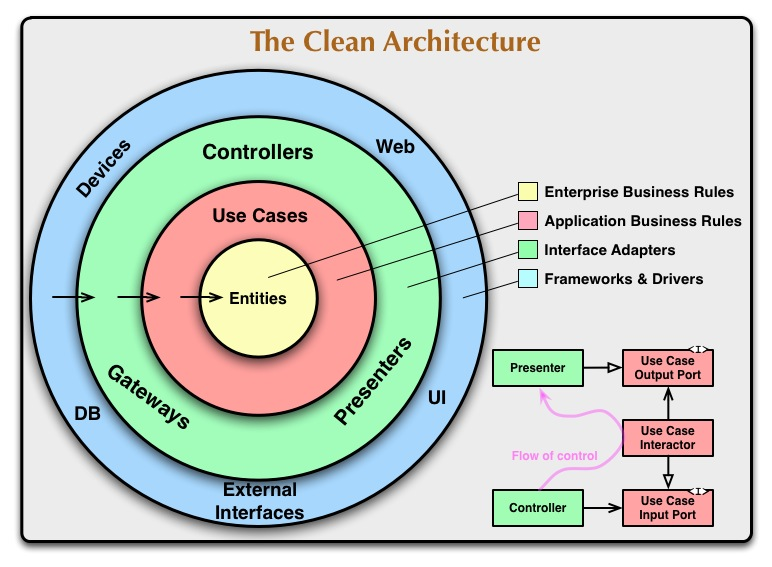
\includegraphics[width=15cm]{clean_architecture.jpg}
    \centering
    \caption{Darstellung der Clean Architecture \cite{martin_clean_architecture}}
    \label{fig:clean_architecture_circles}
\end{figure}


Der innere Kreis repräsentiert dabei den Kern der Anwendung.
Weiter außen liegende Kreise sind konzeptuell weiter vom Kern der Anwendung entfernt.
Zum Beispiel werden Benutzerschnittstelle, Datenbank, Frameworks und ähnliches zum äußersten Kreis zugeordnet.

Die Grundlage der Clean Architecture ist die sogenannte \textbf{Dependency Rule}.
Nach dieser Regel dürfen Abhängigkeiten nur zu weiter innen liegenden Schichten existieren und nicht umgekehrt.
Dadurch bleiben die inneren Schichten komplett unabhängig von den äußeren Schichten und äußere Schichten werden leicht austauschbar.
Um diese Regel umzusetzen können Schnittstellen in inneren Schichten definiert, und in äußeren Schichten implementiert werden (siehe \textit{\hyperref[sec:DIP]{Dependency Inversion Principle}}).
Die \textit{Interface Adapters}-Schicht (oder auch Adapter-Schicht) aus Abbildung \ref{fig:clean_architecture_circles} hat den Zweck, externe Abhängigkeiten möglichst von der eigentlichen Anwendung zu trennen.
In dieser Schicht werden vor allem Datenkonvertierungen von internen zu externen Formaten und umgekehrt durchgefürht.
Das System kann dadurch intern mit einem beliebigen Format arbeiten und ist dementsprechend unabhängig von Datenformaten, die von externen Abhängigkeiten benötigt werden.
Wenn zum Beispiel die Datenbank ausgetauscht werden soll reicht es aus, einen neuen Adapter zu implementieren.
Die eigentliche Kernanwendung muss also nicht verändert werden, wenn externe Komponenten ausgetauscht werden sollen.
Damit ist die Entwicklung flexibler und möglichst technologieunabhängiger System möglich.

\section{Begründung der Clean Architecture}

%TODO: Begründung für Umsetzung der Clean Architecture
%TODO: Erklärung für Umsetzung >= 1 Klasse der Adapterschicht